\label{chap:discussion}



\epigraph{Our imagination is the only limit to what we can hope to have in the future.}{\textit{Charles F. Kettering \\ American inventor, engineer and businessman }}

Firstly, this chapter deals with the conclusions of the study and the future work on study. Secondly, it focuses on the parameters of laser shock peening. Lastly, this chapter describes the experimental equipment used for laser shock peen-ing at the HiLASE centre.

\section{Conclusions of study and future work on study}

Let us recapitulate the goals of this study from the section \hyperref[sec:introduction]{\ref{sec:introduction} Introduction}:

\begin{enumerate}

    \item creating a simulation of a LSP process in CAM software,
    \item developing a post processor for the LSP process, 
    \item generating a program  for the robotic arm controller from simulation,
    \item test simulation of LSP process on actual robotic arm controller.
    
\end{enumerate}

The first goal is described in section  \hyperref[sec:setting_up]{\ref{sec:setting_up} Setting up a curve follow project in RoboDK}, the second goal in section  \hyperref[sec:modifying]{\ref{sec:modifying} Modifying the FANUC R--30iA post processor methods}. The third goal has been achieved in section  \hyperref[sec:example]{\ref{sec:example} Example output of modified FANUC R–30iA post processor} and finally, the test simulation is demonstrated in \hyperref[chap:testing]{Chapter 5 -- Testing}.

This study addresses the problem of modifying a FANUC robotic arm controller post processor for LSP applications. One of the main contributions of our work is to simplify the generation of robotic arm controller programs. In this study, programs are generated using the CAM  program RoboDK. The creation of a robotic arm manually is a tedious process, especially for parts with complex geometries. From an experimental point of view, the contribution lies in testing the programs generated with the help of the CAM program RoboDK.

In the future, the post processor could be improved by incorporating the following features:

\begin{itemize}

    \item implementation of Remote Tool Center Point functionality (RTCP). RTCP ensures a constant robotic arm speed with respect to the surface of the sample in case a static tool is used,

    \item constrain the angular speed of robotic arm joints to a specific limit so that the robotic arm motions will be smoothed.

\end{itemize}
\section{Future direction of the PhD thesis}

This study deals only with one subsystem of the LSP station at HiLASE, namely, creating a robotic arm controller program for a three-dimensional part, and it gives a peek into the future direction of the PhD thesis. The LSP station consists of several subsystems. Figure \ref{fig:subsystems} displays a mind map of the various LSP station subsystems. Each subsystem takes care of a certain aspect of the LSP process. Unfortunately, each subsystem has its unique control software. The ultimate goal of the PhD thesis is to create a  Supervisory Control And Data Acquisition (SCADA) control system to unify the fragmented subsystem's control software. 

\begin{figure}[h]
    \centering
    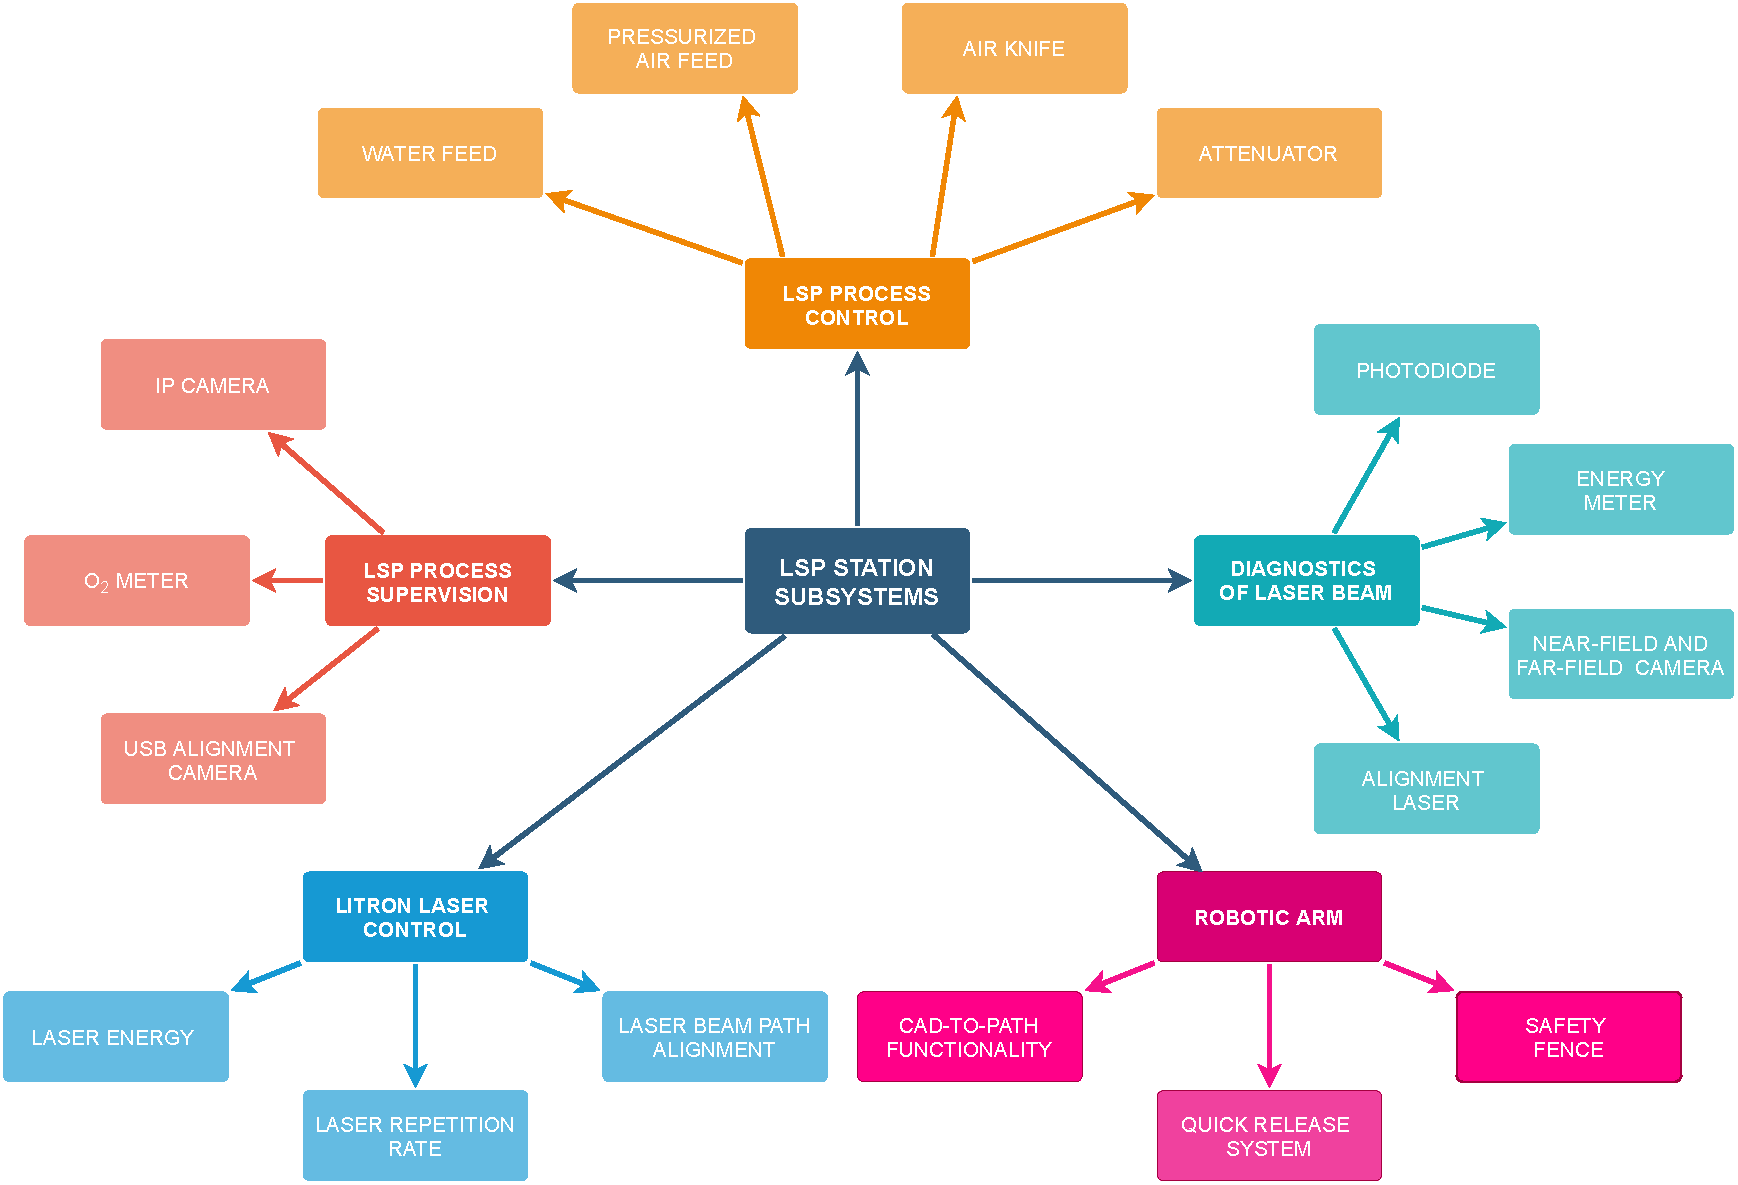
\includegraphics[width=1.0\linewidth]{img/lsp_subsystems.pdf}
    \caption{Mind map of the various LSP station subsystems}
    \label{fig:subsystems}
\end{figure}


The subsystems will be integrated using LabVIEW. LabVIEW (Laboratory Virtual Instrument Engineering Workbench) will be the development environment used in the PhD thesis. LabVIEW uses a graphical notation to create applications instead of lines of text. LabVIEW programs are called Virtual Instruments (VIs). LabVIEW is used for data acquisition, signal processing, and hardware control.

A LabVIEW program consists of the front panel window and the block diagram window. The front panel window contains controls and indicators (i.e., inputs and outputs). The block diagram window contains terminals corresponding to front panel controls and indicators, as well as constants, functions, structures, and wires that connect data from one object to another \cite{bress_2013}.


\subsection{Robotic arm Human-Machine Interface for LSP applications}

The PhD thesis topic is partly investigated in the journal article of MM Science Journal named \href{https://www.mmscience.eu/journal/issues/december-2019/articles/robotic-arm-human-machine-interface-for-laser-shock-peening-applications}{Robotic arm Human-Machine Interface for LSP applications} \cite{bohm_kaufman_brajer_rostohar_2019}. This journal article gives a peek into the future direction of the PhD thesis.  The focus of this article is the development of a robotic arm Human-Machine Interface (HMI) for LSP applications.

Learning to program an industrial robotic arm using a teach pendant has a steep learning curve and requires special training because different robotic arm vendors use different Operating Systems (OS) and different programming languages for their respective teach pendants. It is ineffective and time-consuming to provide every employee with the same level of training required to program a robot application. 

Consequently, there is a need to develop a unifying HMI for the LSP station, which allows the operator to control the process and change the process parameters via a Graphical User Interface (GUI) without the need to learn industrial robotic arm programming. The GUI is developed using LabVIEW and the Digimetrix Fanuc Robotics library for LabVIEW. With the Digimetrix Fanuc Robotics library, the developer can integrate FANUC robotic arms into LabVIEW programs \cite{bohm_kaufman_brajer_rostohar_2019}. 

\subsubsection*{Digimetrix Fanuc Robotics library}

The Digimetrix Fanuc Robotics Library add-on is used to simplify the application development process. The solution incorporating the Digimetrix library is unique compared to standard procedures of robot control from superior systems (PC, PLC, CNC) used in industrial automation because it enables the developer to access all of LabVIEW's capabilities. In this way, advanced measurement and machine control can be integrated into a single LabVIEW application and the developer can tailor the program to his needs. Furthermore, the program is mostly hardware-independent, so the code can be reused.

The Digimetrix Library uses the Fanuc User Socket Messaging Communication Option. Socket messaging enables data exchange between networked robots and a remote computer via (Transmission Control Protocol/Internet Protocol) TCP/IP Sockets. The Transmission Control Protocol (TCP) is intended for use as a highly reliable, host-to-host protocol between hosts in packet-switched computer communications networks. It fits into a layered protocol architecture just above a basic Internet Protocol (IP). The IP provides a way for TCP to send and receive variable-length segments of information enclosed in Internet datagram envelopes. The Fanuc Robotics Library enables the controller to communicate with external or host devices across an Ethernet network. The PC with LabVIEW acts as a client and the robot controller as a server as depicted in Figure \ref{fig:client_server}.

\begin{figure}[h]
    \centering
    
\includegraphics[width=0.8\linewidth]{img/client_server.jpg}
    \caption{Client-server configuration of host PC and robot controller \cite{digimetrix}}
    \label{fig:client_server}
\end{figure}

The advantage of the Digimetrix library is that it offers an extensive number of functions. These functions allow controlling almost every aspect of the robotic arm. It is also deeply integrated into the LabVIEW environment. The disadvantage of this library is that the developer must be familiar with LabVIEW, at least on a fundamental level. Another disadvantage of the library is that TCP/IP itself does not support real-time operation \cite{digimetrix}.




